\documentclass[9pt]{beamer}
\usepackage[utf8]{inputenc}
\usepackage{MnSymbol,wasysym}
\usepackage{tikz}
\usetheme{Antibes}
\usecolortheme{whale}
\usepackage{minted}
\usepackage{color}
\definecolor{lightgray}{rgb}{.9,.9,.9}
\definecolor{darkgray}{rgb}{.4,.4,.4}
\definecolor{purple}{rgb}{0.65, 0.12, 0.82}
\definecolor{applegreen}{rgb}{0.55, 0.71, 0.0}
\definecolor{azure(colorwheel)}{rgb}{0.0, 0.5, 1.0}
\definecolor{awesome}{rgb}{1.0, 0.13, 0.32}
\definecolor{ao(english)}{rgb}{0.0, 0.5, 0.0}
\definecolor{darkmidnightblue}{rgb}{0.0, 0.2, 0.4}
\usetikzlibrary{matrix,backgrounds}

\title[CS639A Software Debloating Techniques : Course Project Presentation] %optional
{Is Software Debloating really effective?}

\author[Amit Kumar, Sumit Lahiri] % (optional, for multiple authors)
{Amit Kumar, 20111012\inst{1}, Sumit Lahiri, 19111274\inst{1}}

\institute[IIT Kanpur] % (optional)
{
	\inst{1}%
	Computer Science \& Engineering Dept.\\
	Indian Institute Of Technology, Kanpur
}
\subtitle{Analysis \& Comparison Report}
\date[August 2019 - April 2024] % (optional)

\begin{document}

\definecolor{applegreen}{rgb}{0.55, 0.71, 0.0}
\definecolor{azure(colorwheel)}{rgb}{0.0, 0.5, 1.0}
\definecolor{awesome}{rgb}{1.0, 0.13, 0.32}
\definecolor{ao(english)}{rgb}{0.0, 0.5, 0.0}
\definecolor{darkmidnightblue}{rgb}{0.0, 0.2, 0.4}
\frame{\titlepage}

\begin{frame}
	\frametitle{What is Software Debloating?}
	\begin{block}{The Problem}
		\begin{itemize}
			\pause
			\item Multitude of options for a software package with flags [--stats, --debug] etc.
			\pause
			\item Do we need all the options and API calls when running for a specific purpose?
			\pause
			\item What if some options or flags are never used?
		\end{itemize}
	\end{block}
	\pause
	\begin{block}{Solution}
	\begin{itemize}
		\pause
		\item To selectively remove such code sections that are not needed for current execution.
		\pause
		\item Exponentially large number of specific binaries produced, almost all possible combinations!!
	\end{itemize}
	\end{block}
\end{frame}
\begin{frame}
	\frametitle{How Software Debloating Works?}
	\pause
	\begin{block}{Hinderances}
		\begin{itemize}
			\pause
			\item  Execution environment modelling.
			\pause
			\item Decide when to remove BBs from the Control Flow Graph ?
			\pause
			\item Can we do better ?
			\pause
		\end{itemize}
	\end{block}
	\begin{block}{Rescue}
		\begin{itemize}
			\pause
			\item Debloating tools to rescue !! 
			\pause
			\item Source Code [\texttt{C} or \texttt{C++}] files
			\pause
			\item Specification : What is desired? What all must be executed in the current execution context?
			\pause
			\item Selectively remove those code sections that dont need to be executed as per the specifications provided.
		\end{itemize}
	\end{block}
\end{frame}
\begin{frame}[fragile]
	\frametitle{Simple Example}
	\begin{minted}{c++}
	#include <stdio.h>
	void run(int a) {
		if (a > 90) {
			printf("%d\n", a);
		}
	}
	long long int add(int a, int b) 	{ return a + b; }
	long long int sub(int a, int b) 	{ return a - b; }
	int main(int argc, char *argv[]) {
		int c = 0;
		c = -500;
		if (c > 0) {
			run(c);
			add(c, c + 1);
		} else {
			sub(c + 90, c);
		}
		return 0;
	}
	\end{minted}
\end{frame}
\begin{frame}[fragile]
	\frametitle{After Chisel Tool}
	\texttt{Blank Oracle File}
	\begin{minted}{c++}
	#include <stdio.h>
	
	int main(int argc, char *argv[]) {
		int c = 0;
		
		return 0;
	}
	\end{minted}
\end{frame}
\begin{frame}[fragile]
	\frametitle{Before : OCCAM Run}
	\begin{minted}{c++}
		Statistics for  before specialization
		[CFG analysis]
		4 Number of functions
		0 Number of specialized functions
		0 Number of bounced functions added by devirt
		9 Number of basic blocks
		52 Number of instructions
		4 Number of direct calls
		1 Number of external calls
		0 Number of assembly calls
		0 Number of indirect calls
		0 Number of unknown calls
		0 Number of loops   
		0 Number of bounded loops
		[Memory analysis]
		22 Number of memory instructions
		22 Statically safe memory accesses
		0 Statically unknown memory accesses
	\end{minted}
\end{frame}
\begin{frame}[fragile]
	\frametitle{After : OCCAM Run}
	\begin{minted}{c++}
		Statistics for  after specialization
		[CFG analysis]
		2 Number of functions
		0 Number of specialized functions
		0 Number of bounced functions added by devirt
		5 Number of basic blocks
		25 Number of instructions
		2 Number of direct calls
		1 Number of external calls
		0 Number of assembly calls
		0 Number of indirect calls
		0 Number of unknown calls
		0 Number of loops   
		0 Number of bounded loops
		[Memory analysis]
		7 Number of memory instructions
		7 Statically safe memory accesses
		0 Statically unknown memory accesses
	\end{minted}
\end{frame}
\begin{frame}
	\frametitle{Our Project}
	\pause
	\begin{block}{Objectives}
	\begin{itemize}
		\pause
		\item Understanding of debloating techniques.
		\pause
		\item Run state-of-the-art debloating tools against benchmarks for comparison between different approaches and techniques
		\pause
		\item Implementation of \texttt{DeepOCCAM} from \texttt{OCCAM} based on \texttt{DeepOCCAM} Paper. 
	\end{itemize}
\end{block}
	\begin{block}{Tools}
		\begin{itemize}
			\pause
			\item \texttt{OCCAM} : Automated Software Winnowing
			\pause
			\item \texttt{Trimmer} : Input Specialization, Specialized Loop Unrolling, Constant Propagation. 
			\pause
			\item \texttt{Chisel} : Reinforcement Learning based Delta Debugging on a set of Tests.
			\pause
			\item \texttt{DeepOCCAM} : An extension to \texttt{OCCAM}, based on Reinforcement Learning based Specialization Action. 
		\end{itemize}
	\end{block}
\end{frame}
\begin{frame}
	\frametitle{Implementation}
	\pause
	\begin{block}{Pipelines}
		\begin{itemize}
			\pause
			\item \texttt{OCCAM}
			\pause
			\item \texttt{OCCAM-T} : A modified run of OCCAM with \texttt{--unroll-loop, --ipdce, specialize=true}
			\pause
			\item \texttt{Chisel} : Modified to dump chunks and other metrics data
			\pause
			\item \texttt{DeepOCCAM} : Developed from base \texttt{OCCAM} tool. 
		\end{itemize}
	\end{block}
\end{frame}
\begin{frame}[fragile]
	\frametitle{Diagrams}
	\begin{block}{Chisel}
			\begin{figure}[H]
				\centering
				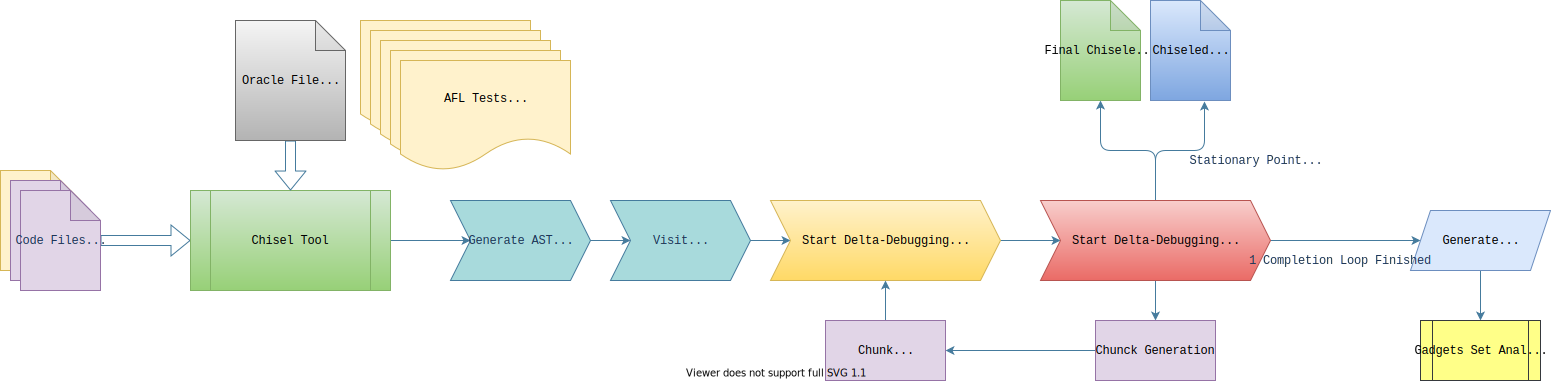
\includegraphics[width=1\linewidth]{imgs/chisel-pipeline.png}
				\caption{\textbf{Chisel Pipeline} : Setup \texttt{Chisel} runs on \texttt{Chisel-Benchmarks} \& other examples}%
				\label{fig:plant}
			\end{figure}
	\end{block}
\end{frame}
\begin{frame}[fragile]
	\frametitle{Diagrams}
	\begin{block}{OCCAM}
		\begin{figure}[H]
		\centering
		\includegraphics[width=1\linewidth]{imgs/occam-pipeline.png}
		\caption{\textbf{OCCAM Pipeline} : Setup \texttt{OCCAM} runs on \texttt{OCCAM-Benchmarks} \& other examples}%
		\label{fig:plant}
		\end{figure}
	\end{block}
\end{frame}
\begin{frame}[fragile]
	\frametitle{Diagrams}
	\begin{block}{Trimmer}
		\begin{figure}[H]
			\centering
		\includegraphics[width=1\linewidth]{imgs/occam-modified-trimmer.png}
		\caption{\textbf{Trimmer Runs} : Setup \texttt{Trimmer} runs on \texttt{OCCAM-Benchmarks} only}%
		\label{fig:plant}
		\end{figure}
	\end{block}
\end{frame}
\begin{frame}[fragile]
	\frametitle{Diagrams}
	\begin{block}{DeepOCCAM}
		\begin{figure}[H]
			\centering
		\includegraphics[width=0.8\linewidth]{imgs/deepoccam-pipeline.png}
		\label{fig:plant}
		\end{figure}
	\end{block}
\end{frame}
\begin{frame}[fragile]
	\frametitle{Static Analysis}
	\begin{block}{httpd program}
		\begin{figure}[H]
			\centering
			\includegraphics[width=0.8\linewidth]{imgs/static_analysis_1.png}
			\label{fig:plant}
		\end{figure}
	\end{block}
\end{frame}
\begin{frame}[fragile]
	\frametitle{Static Analysis}
	\begin{block}{curl program}
		\begin{figure}[H]
			\centering
			\includegraphics[width=0.8\linewidth]{imgs/static_analysis_2.png}
			\label{fig:plant}
		\end{figure}
	\end{block}
\end{frame}
\begin{frame}[fragile]
	\frametitle{Dynamic Analysis}
	\begin{block}{Chisel Runs}
		\begin{figure}[H]
			\centering
			\includegraphics[width=0.8\linewidth]{imgs/dynamic_analysis_1.png}
			\label{fig:plant}
		\end{figure}
	\end{block}
\end{frame}
\begin{frame}[fragile]
	\frametitle{Dynamic Analysis}
	\begin{block}{Full Comparison}
		\begin{figure}[H]
			\centering
			\includegraphics[width=0.8\linewidth]{imgs/dynamic_analysis_2.png}
			\label{fig:plant}
		\end{figure}
	\end{block}
\end{frame}
\begin{frame}[fragile]
	\frametitle{Chisel Learning}
	\begin{block}{Plots}
		\begin{figure}[H]
			\centering
			\includegraphics[width=0.8\linewidth]{imgs/chisel_tool_learning.png}
			\label{fig:plant}
		\end{figure}
	\end{block}
\end{frame}
\begin{frame}
	\frametitle{Conclusion}
	\begin{block}{Insights \& Closing Remarks}
		\begin{itemize}
			\pause
			\item Did Chisel Won? \pause No !!, \pause 14 hrs to run \texttt{bzip2}, \pause 1 day to run \texttt(uniq)
			\pause
			\item How to decide which tool to use based on the comparison we showed?
			\pause
			\item Depends on our objective. 
			\pause
			\item Recommend \texttt{Chisel} : With AFL Fuzzing or EGT [Symbolic Execution]
			\pause
			\item Recommend \texttt{OCCAM Variants} : Writing manifest simple!, less effective on gadgets reduction.
		\end{itemize}
	\end{block}
\end{frame}
\end{document}